% Canonical, editable manuscript. All prose, equations, and tables are in this file.
% Build: latexmk -pdf -interaction=nonstopmode -halt-on-error mainj.tex
% Anonymous development draft; main-study efficacy remains untested.
\documentclass[runningheads,orivec]{llncs}
\usepackage[T1]{fontenc}
\usepackage[utf8]{inputenc}
\usepackage{newtxtext}
\usepackage[varvw]{newtxmath}
\usepackage{graphicx}
\usepackage{booktabs}
\usepackage{float}
\usepackage{microtype}
\usepackage[hidelinks]{hyperref}
\hypersetup{pdfauthor={Anonymous},pdftitle={Diagnosing and Correcting Unstable Generative Underwater Acoustic Repair},pdfsubject={Anonymous development study; targeted correction and operational limitations}}

\begin{document}
\raggedbottom
\title{Diagnosing and Correcting Unstable\texorpdfstring{\\}{ }Generative Underwater Acoustic Repair}
\titlerunning{Diagnosing Generative Underwater Acoustic Repair}
\author{Anonymous submission}
\authorrunning{Anonymous}
\institute{}
\maketitle

\begin{abstract}
Trustworthy acoustic evidence supports object labeling and equipment decisions. We study repairing known gaps in public underwater vessel recordings while keeping estimated samples marked. An initial diffusion pilot exposes a specific failure: converting predicted noise into sound amplifies squared prediction error by approximately $4.12\times10^8$ at the terminal diffusion step. Precision and clipping controls isolate the problem. A matched 5,000-update intervention uses established velocity prediction to remove that conversion singularity. On four diagnostic recordings, full-precision gap NMSE falls from $5.18\times10^6$ to 1.03 without clipping or skipping the terminal step. Across 192 reused development groups, acoustic error also decreases. On the 64 reserved development cases, first-draw combined error Q falls from 0.412 to 0.308, a 25\% reduction, although the learned baseline remains better at 0.239. The correction therefore resolves the observed numerical failure without establishing sufficient acoustic usefulness. Three spectrogram and listening examples connect the comparison to excess energy, frequency structure, and low-tone continuity; an analysis-window comparison illustrates the tradeoff between timing and frequency detail. The original release rule declines every generative proposal, and no new rule is calibrated for the corrected model. This study demonstrates an inspectable diagnose--correct--verify workflow. Object identification, physical equipment control, and a reasoning agent remain downstream proposals requiring separate evaluation.
\keywords{Generative AI \and Passive acoustics \and Audio inpainting \and AI abstention \and Operator decision support}
\end{abstract}

\section{From acoustic evidence to labels and settings}

An acoustic or sonar operator needs to answer three questions: what was measured, which label is justified, and would a different setting improve the evidence? Ship recordings contain low-frequency components and broadband energy \cite{veirs}. Figure~\ref{fig:configuration} separates a measured cue from a supplied vessel label and demonstrates two analysis settings. A component near 78 Hz is a feature; it does not by itself identify a tanker or another object.

\begin{figure}[!ht]
\centering
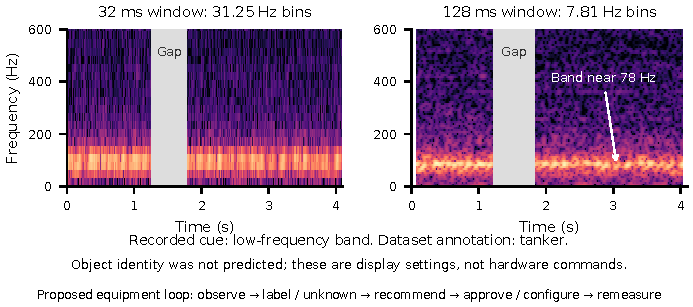
\includegraphics[width=\linewidth]{operator_configuration.pdf}
\caption{Same available recording: 32/4 ms and 128/16 ms window/hop settings. Longer windows give finer frequency bins but blur timing and exclude a wider interval around missing samples (gray). Every frame touching the gap is omitted. Brightness shows relative power, with a common $-60$ to 0 dB scale. ``Tanker'' is the dataset annotation, not a model prediction. Equipment-control steps in the proposed workflow were not tested.}
\label{fig:configuration}
\end{figure}

\emph{Generative AI} proposes missing sound; \emph{AI abstention} declines a generative proposal when the release rule fails. A \emph{provenance mask} marks measured versus filled samples, even when a baseline fill is used. These concepts protect the distinction between data and suggestions upstream of labeling and configuration.

The pilot uses public single-hydrophone recordings, artificial gaps, and 8 kHz audio below 4 kHz. It includes no submarine recordings, array processing, active echoes, or operator trial. Actual calibration and final-test outcomes remain unopened; amplitudes are relative, not calibrated sound-pressure levels.

The engineering question is whether an unsuccessful generator can reveal a correctable failure mechanism. We separate two tests: removing numerical error amplification, and improving reconstructed sound against a fixed baseline. A targeted follow-up changes the diffusion prediction target while retaining the architecture, training data, and update budget. This connects a reproducible failure trace to a specific intervention, with separate checks on stability and acoustic usefulness.

\section{Prior work and the recordings used}

UniqueShip addresses leakage in acoustic ship classification \cite{uniqueship}. Underwater spectrogram inpainting is already studied by Tembo et al. \cite{tembo}; their metadata were verified, but primary full text was unavailable. General-audio diffusion inpainting \cite{moliner}, DiffWave \cite{diffwave}, CSDI conditioning \cite{csdi}, inpainting uncertainty \cite{cohen}, risk calibration \cite{ltt}, and similarity guidance \cite{simdps} are established components. Velocity prediction is an established diffusion parameterization \cite{salimans}; our contribution is a controlled diagnostic application to this acoustic failure, not a new diffusion formulation.

The audited UniqueShip v1 twelve-class, five-hours-per-class archive has 43,208 mono PCM32 recordings at 32 kHz, totaling 60.008 hours; headers differ from the website's 20 kHz description. Twelve clips are shorter than the 4.096 s crop. Table~\ref{tab:1} preserves the first official test split, validation where feasible, and separates generator fitting G, quality-checker fitting D, development V, and calibration C by source/vessel group.

\begin{table}[htbp]
\caption{Audited source partitions; counts describe available data, not evaluated outcomes.}
\label{tab:1}
\centering\small
\begin{tabular*}{\linewidth}{@{\extracolsep{\fill}}lrrr@{}}
\toprule

\textbf{Partition} & \textbf{Sources} & \textbf{Groups} & \textbf{Pilot use} \\

\midrule

G & 26,321 & 2,996 & 1,440 sources \\

D & 3,962 & 467 & 200 groups \\

V & 4,445 & 400 & 200 groups \\

C & 4,003 & 547 & Unopened \\

Test & 4,477 & 610 & Unopened \\

\bottomrule
\end{tabular*}
\end{table}

All source descendants remain grouped; background uses hydrophone/date, with unknown devices pooled by date. Hash checks found no duplicates; timestamps found no cross-partition overlap or separation below 60 s. Yet 1,332/1,522 dates span partitions and parent/session IDs are unavailable, so environmental independence is unproven. Exhaustive shifted-duplicate detection was not performed. V/D lack pilot-vessel examples; C also lacks dredger; test lacks dredger and supports eleven classes. No identification accuracy is reported. Complete audio is resampled before artificial masking.

\section{Generate, check, select, and keep the gap marked}

\textbf{Generate:} refine random noise in the gap into four possible fills. \textbf{Check:} rebuild two deliberately hidden nearby segments with known originals. \textbf{Select:} predict error relative to baseline B, then apply a release rule. \textbf{Mark:} retain the missing-sample flag. B is a deterministic learned restorer, also machine learning; P denotes the full rule's output.

For mask $m$ and input $y=m\odot x$, hidden values are erased before processing. Mean/RMS scaling uses observed samples only, with a training-fixed floor. Every generation step copies observations back; final inverse scaling preserves original observations exactly:
\begin{equation}
\Pi_y(z)=m\odot y+(1-m)\odot z.\label{eq:projection}
\end{equation}
Gaps are 50, 100, 250, or 500 ms with at least 0.75 s context per side. Training uses one gap 80\% of the time, otherwise two. Four proposals plus two known-audio checks use 32 DDIM steps each \cite{ddim}, totaling 192 evaluations. Each check hides its samples before recomputing normalization; references and labels never enter inference.

B minimizes development Q against bidirectional autoregressive orders 16/32/64/128. A histogram gradient-boosting regressor fits proposal-minus-B error $\Delta Q$ on 200 equally weighted D groups. Its 18 features summarize proposal disagreement, differences from B, boundaries, and known-audio errors. The lowest predicted error selects the proposal. Simpler duration-only and disagreement-only gates retain this selector.

\section{Implementation and what the error scores mean}

The DiffWave adaptation \cite{diffwave} has 64 channels, 36 residual layers, dilations 1--2048 repeated three times, 2,717,697 parameters, and a 3.071 s receptive field. A 1,000-step cosine schedule \cite{nichol}, seed 17, batch 16, and 5,000 updates use 1,440 G sources (about two hours). The same-backbone baseline trains for 2,500 updates with masked MAE plus 0.5 times multiresolution spectral convergence. Training takes 29.3/17.9 minutes on one RTX 4090, with 2.56 GiB peak allocation each.

A reduced-width, 16-source diagnostic lowers loss but does not establish near-zero memorization after 2,000 updates. CUDA checkpoint restoration reproduces the next batch, RNG, loss, and parameters exactly. A 200-crop, six-output metric check has finite scores and zero observed-sample drift.

Unbounded DDIM fails on four G-only cases: $\bar\alpha_{999}=2.43\times10^{-9}$ amplifies prediction error to gap NMSE in the millions. Clipping alone leaves Q saturated at one. Before V outcomes, a recorded amendment starts at $t=934$, the last timestep with $\bar\alpha\geq0.01$, and clips clean predictions at the G-derived bound $\pm5.897$. Noise is recomputed after clipping; observations are never clipped. Gaussian initialization at this nonterminal step introduces a train--inference mismatch \cite{lin}; the amended sampler is approximate.

\begin{equation}
Q=\tfrac12\min\!\left(\frac{\mathrm{NMSE}_{\mathrm{gap}}}{4},1\right)+\tfrac12\min\!\left(\frac{\mathrm{SC}_{\mathrm{gap}}}{2},1\right).\label{eq:quality}
\end{equation}

NMSE measures waveform mismatch relative to reference energy; SC measures frequency-magnitude mismatch. Lower is better for both and their combined Q. SC averages gap-only convergence at FFT sizes 64/128/256 with periodic Hann windows, quarter-window hops, and no centered padding. A ``worse'' fill exceeds B's Q by over 0.02: a reconstruction criterion, not an identification or safety score.

The release rule seeks at most 10\% worse fills among accepted proposals. V freezes at most nine nonpositive cutoffs. For $n$ acceptances and $e$ worse fills, the one-sided Clopper--Pearson bound uses level $1-0.05/M$ across $M$ cutoffs. A cutoff qualifies only if its bound is $\leq0.10$; $n=0$ gives one. Otherwise generative release is disabled. This requires independent, identically distributed groups and a frozen policy \cite{ltt}, not arbitrary site changes.

\section{Original pilot: the rule declines every AI proposal}

V assigns 64 groups each to tuning, practice calibration, and reserved-case evaluation, with eight unused; the first 32 tuning groups also monitor training. B wins tuning Q (0.218; AR128: 0.229). Even choosing the best proposal with the reference, only 5/64 (7.8\%) improve Q by $\geq0.02$, below the 20\% requirement. At 64 steps this remains 5/64 while latency rises from 1.28 to 2.48 s. We retain 32 steps and stop the main study.

\begin{table}[htbp]
\caption{One case per reserved development group ($n=64$). Lower error is better. AI use is the fraction receiving a diffusion proposal; Worse is the fraction with Q over 0.02 above B. Calls count diffusion evaluations; B needs one restoration pass. Velocity rows are the follow-up in Sect.~\ref{sec:correction}, without a release gate.}
\label{tab:2}
\centering\small
\begin{tabular*}{\linewidth}{@{\extracolsep{\fill}}lrrrrr@{}}
\toprule

\textbf{Output} & \textbf{Error Q} & \textbf{NMSE} & \textbf{AI use} & \textbf{Worse} & \textbf{Calls} \\

\midrule

Zero fill & 0.375 & 1.000 & 0.00 & --- & 0 \\

Linear interpolation & 0.314 & 1.021 & 0.00 & --- & 0 \\

Baseline fill B & 0.239 & 0.713 & 0.00 & --- & 0 \\

One AI proposal (C1) & 0.412 & 2.274 & 1.00 & 0.891 & 32 \\

Central of four (C2) & 0.404 & 1.949 & 1.00 & 0.891 & 128 \\

Always use selected AI (C3) & 0.349 & 1.460 & 1.00 & 0.812 & 192 \\

Checked output P & 0.239 & 0.713 & 0.00 & 0.000 & 192 \\

\midrule

Velocity: old sampler & 0.318 & 1.313 & 1.00 & 0.781 & 32 \\

Velocity: one draw & 0.308 & 1.251 & 1.00 & 0.750 & 32 \\

Velocity: central of four & 0.295 & 1.255 & 1.00 & 0.703 & 128 \\

\bottomrule
\end{tabular*}
\end{table}

All four gates test cutoff zero: 0/64 practice-calibration acceptances give bound one. No cutoff qualifies, disabling the final gate. Always using the selected AI proposal worsens 52/64 gaps; P uses B throughout. Accepted-proposal risk is undefined. This stopping result motivates a targeted correction before further release-policy evaluation.

Gap NMSE is 0.713 for B/P and 1.460 for C3, versus full-window 0.038/0.074; unchanged context dilutes error. C3's 99th-percentile gap NMSE is 6.944 versus B's 2.596. Observed drift is zero. A 2,000-draw group bootstrap gives P-minus-C3 Q $-0.110$ (95\% interval $-0.130$ to $-0.089$); balancing 63 dates gives $-0.112$ ($-0.132$ to $-0.091$), a different estimand. Both are exploratory.

\section{From a failure trace to a targeted correction}
\label{sec:correction}

\textbf{Isolate the mechanism.} On a missing coordinate, write the forward-noised signal as $z_t=\sqrt{\bar\alpha_t}x_0+\sqrt{1-\bar\alpha_t}\epsilon$. The original network predicts noise $\hat\epsilon_\theta$. For the same $z_t$, its clean-signal estimate and error satisfy
\begin{equation}
\begin{aligned}
\hat x_0^{\epsilon}&=\frac{z_t-\sqrt{1-\bar\alpha_t}\hat\epsilon_\theta}{\sqrt{\bar\alpha_t}},\\
\|\hat x_0^{\epsilon}-x_0\|_2^2&=\frac{1-\bar\alpha_t}{\bar\alpha_t}\|\hat\epsilon_\theta-\epsilon\|_2^2.
\end{aligned}\label{eq:amplification}
\end{equation}
At $t=999$, the squared-error multiplier is approximately $4.12\times10^8$. A small error in predicted noise can therefore produce a very large waveform error. This is local error propagation at a known forward-noised state; it does not by itself model the full sampling trajectory.

The saved four-source G diagnostic separates this mechanism from precision and amplitude bounding. With the same model, sources, masks, and noise seed, full-precision sampling also fails, so reduced precision alone cannot explain the problem. Clipping removes extreme amplitude but leaves Q saturated at one. Starting later reduces the amplification but changes the initialization assumption. These controls explain why the original numerical amendment enabled evaluation without establishing useful repair.

\textbf{Change the prediction coordinates.} Following Salimans and Ho \cite{salimans}, train the same network to predict a velocity target and recover both clean signal and noise through a rotation:
\begin{equation}
\begin{aligned}
v_t&=\sqrt{\bar\alpha_t}\epsilon-\sqrt{1-\bar\alpha_t}x_0,\\
\hat x_0^{v}&=\sqrt{\bar\alpha_t}z_t-\sqrt{1-\bar\alpha_t}\hat v_\theta,\\
\hat\epsilon^{v}&=\sqrt{1-\bar\alpha_t}z_t+\sqrt{\bar\alpha_t}\hat v_\theta.
\end{aligned}\label{eq:velocity}
\end{equation}
Now the squared clean-signal error equals $(1-\bar\alpha_t)\|\hat v_\theta-v_t\|_2^2$ at a fixed state: its multiplier is at most one. The conversion avoids division by the small signal coefficient. ``Velocity'' names a mathematical diffusion coordinate, not vessel speed or a physical acoustic velocity measurement.

The observed-sample mask $m$ confines the training objective to erased coordinates; the norms sum across missing samples in each microbatch:
\begin{equation}
\mathcal L_v=\mathbb E_{t,\epsilon}\!\left[
\frac{\|(1-m)\odot(\hat v_\theta-v_t)\|_2^2}{\|1-m\|_1}
\right].\label{eq:velocity_loss}
\end{equation}
This also changes the implied weighting of clean-signal error across noise levels: velocity loss weights it by $1/(1-\bar\alpha_t)$, whereas noise loss uses $\bar\alpha_t/(1-\bar\alpha_t)$. The intervention therefore changes both prediction coordinates and training emphasis; we do not attribute any acoustic gain to conversion arithmetic alone.

\textbf{Test one fixed correction.} Before the new run, we record one 5,000-update, seed-17 intervention with the same 1,440 G sources, initialization, crop/mask/noise random streams, batch size, optimizer, EMA, and cosine schedule. The final checkpoint is fixed in advance. The primary sampler starts at 999 without clipping; a second velocity sampler retains the original 934/clipping settings to separate sampler effects. All use 32 steps. The unchanged schedule has near-zero, not exactly zero, terminal signal power; no zero-SNR rescaling is claimed \cite{lin}.

We reuse all 192 V groups with identical gaps and four candidate seeds, reporting the original tuning, practice-calibration, and reserved-development groups separately. First draw and spectral medoid are usable selection rules; reference-based best-of-four remains an oracle. Pairing is by recording group, with 2,000 bootstrap draws for exploratory intervals. This follow-up was motivated by inspected V results and is not a new confirmatory test. The original quality predictor and gate are not transferred to the new generator; actual C/test outcomes remain unopened.

\begin{figure}[!ht]
\centering
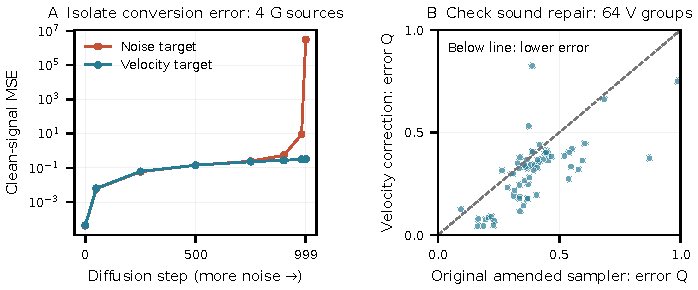
\includegraphics[width=\linewidth]{velocity_correction.pdf}
\caption{A: clean-signal error at known forward-noised states, averaged over the same four G recordings; solid/dashed curves use full/reduced precision. B: fixed first draws on the same 64 tuning groups; points below the diagonal favor the correction. A diagnoses numerical amplification; B measures acoustic repair. The original model in B uses its amended sampler.}
\label{fig:correction}
\end{figure}

\textbf{Verify the fix and locate the next bottleneck.} Figure~\ref{fig:correction} separates numerical and acoustic effects. On the four G cases, full-precision gap NMSE changes from $5.18\times10^6$ (original terminal sampler), to 22.55 (clipping only), to 1.84 (original amended sampler), to 1.03 (velocity, terminal and unclipped). Matching end-of-training RNG states verifies the paired training streams. The added training and evaluation take 29.2 and 7.3 minutes on the same RTX 4090.

First-draw Q improves from 0.395 to 0.309 on tuning, 0.416 to 0.307 on practice calibration, and 0.412 to 0.308 on reserved development. For the latter, the paired change is $-0.103$ (exploratory 95\% interval $-0.129$ to $-0.077$); balancing its 63 dates gives $-0.104$ ($-0.132$ to $-0.077$). Table~\ref{tab:2} separates the new target with the old sampler from the terminal sampler and four-draw medoid. Observed samples remain exact. Yet the terminal model's best-of-four improves on B by 0.02 in only 7/64 tuning groups (10.9\%), still below the unchanged 20\% trigger. Numerical amplification is now controlled; matching the missing acoustic structure is the remaining measured limitation. Further acoustic modeling should precede a new release-policy study.

\section{Three practical questions about a repaired recording}

Figure~\ref{fig:acoustic_cases} retains the original pipeline's best/worst C3-minus-B Q among 64 reserved V cases (A/B), plus the lowest observed-context spectral flatness among 17 cases with 500 ms gaps (C). These post hoc anecdotes were selected before the correction and now include its fixed first draw. C3 uses learned selection, so the figure illustrates behavior under different selection rules; Table~\ref{tab:2} also provides matched first-draw comparisons.

\begin{figure}[!ht]
\centering
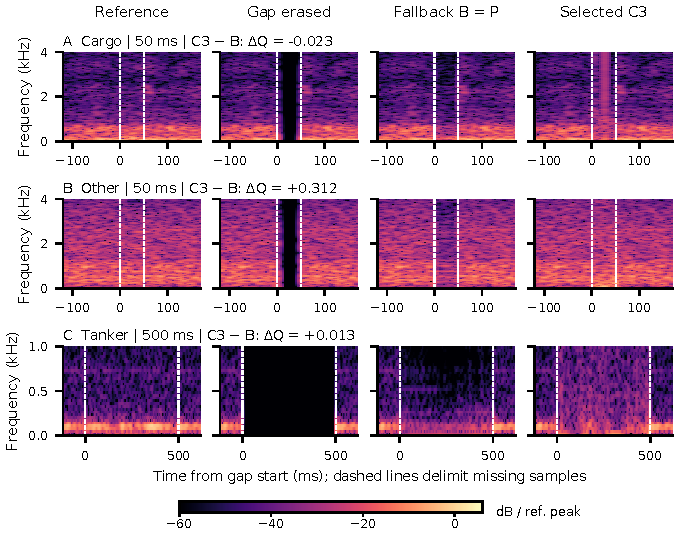
\includegraphics[width=\linewidth]{acoustic_case_studies.pdf}
\caption{Complete reference, baseline B, original selected C3, and the corrected model's first draw. Dashed lines bound the gap. Brightness shows relative energy, with one scale per row; C zooms to 0--1 kHz. The 32 ms Hann windows (4 ms hop) can straddle boundaries. The reference is unavailable during real data loss. The original rule uses B; the corrected proposals have no release gate.}
\label{fig:acoustic_cases}
\end{figure}

\noindent\textbf{A: Better score, same sound pattern?} For cargo (50 ms gap), C3 lowers Q from B's 0.364 to 0.340, yet frequency error rises from 0.727 to 0.765. The correction gives Q 0.343 and frequency error 0.699. Different error measures capture different improvements; none establishes a more reliable vessel label.

\noindent\textbf{B: Louder fill, stronger real event?} For the other-vessel class (50 ms), C3's gap RMS is 3.38 dB above the reference. The correction is 1.73 dB below and lowers Q from 0.590 to 0.354; B still scores 0.278. This illustrates reduced excess energy, but generated level alone cannot justify an acquisition-gain change.

\noindent\textbf{C: Did the low tone stop?} For tanker (500 ms), the reference's component near 78 Hz continues. B and C3 lower gap RMS by 14.48 and 7.13 dB; the correction is only 1.14 dB below reference, yet Q rises from C3's 0.364 to 0.412. Recovering level does not recover the waveform. Neither a weak fill nor a generated tone proves silence or object identity. Figure~\ref{fig:configuration} offers finer frequency detail in the \emph{recorded} context.

\section{What the pilot cannot establish}

The original pipeline's seven synthetic conditions have 100 realizations each: tonal continuation, chirp, onset, offset, colored background, and two hidden-event targets. Paired targets share observations/seeds but differ by a fully hidden transient. All 400 method--pair comparisons produce identical outputs. At event-projection threshold 0.5, each method misses all 100 inserted events and makes no false-event decision on absent counterparts. These controlled signals show missing evidence, not validated ocean propagation or recoverable hidden events; they were not rerun for the correction.

\begin{table}[htbp]
\caption{Conditions outside the usual training setup, with 20 V sources each. The fixed rule uses B throughout; zero AI use does not validate a risk bound in new conditions.}
\label{tab:3}
\centering\small
\begin{tabular*}{\linewidth}{@{\extracolsep{\fill}}lrrr@{}}
\toprule

\textbf{Condition} & \textbf{Cases} & \textbf{AI use} & \textbf{Error Q(P)} \\

\midrule

750 ms gap & 20 & 0.00 & 0.274 \\

1,000 ms gap & 20 & 0.00 & 0.299 \\

Four 50 ms gaps & 20 & 0.00 & 0.188 \\

Short context & 20 & 0.00 & 0.254 \\

Level/spectrum shift & 20 & 0.00 & 0.208 \\

\bottomrule
\end{tabular*}
\end{table}

The fixed-rule checks in Table~\ref{tab:3} change gap length, packet geometry, context, or smooth level/spectrum. Multiple gaps and insufficient probe context trigger predetermined fallback. Outcomes do not retune the model, normalization, or cutoff.

An isolated compatibility run uses Moliner and Välimäki's published EMA checkpoint \cite{moliner} on eight fixed V groups without fine-tuning. Its 22.05 kHz, 184,184-sample configuration is retained. Only masked observations are resampled; the gap expands by 12 input samples, unknown padding is excluded from guidance, and final observed samples are copied exactly. First-run Q/SC are 0.655/1.256; replay Q is 0.654, not bitwise reproducible on the recorded CUDA stack. This is a small adapted compatibility check, not benchmark superiority.

One short training seed, small V subsets, shared environments, and follow-up reuse of inspected outcomes limit interpretation. The original sampler is approximate; the correction retains the same near-zero-terminal schedule. Three-seed training, six-draw medoid C4, one 192-step draw C5, waveform RePaint C6 \cite{repaint}, independent classifier, and VLIZ evaluation were not run. Tonal/onset metrics were not pre-frozen. The planned held-out goals---25\% coverage, 25\% relative harm reduction, better ranking, Q/classifier noninferiority, and observation consistency---remain untested together. Zero observed-sample drift is an implementation check.

\section{Toward labels, equipment decisions, and a review agent}

The proposed loop is \textbf{inspect, label or retain unknown, recommend settings, approve/configure, and remeasure}. Labels need source and status: supplied annotation, model hypothesis, or operator-confirmed identification. Correct labeling requires an independently evaluated model, measuring mislabels and unknown responses on original versus repaired inputs. Reconstruction Q cannot replace identification accuracy.

Figure~\ref{fig:configuration} demonstrates analysis settings offline: 32 ms emphasizes timing; 128 ms gives finer frequency bins but spreads uncertainty around gaps. Physical configuration, such as acquisition gain or sample rate, would require instrument capabilities, allowed settings, operator approval, and a new measurement to check the effect. No hardware control or configuration benefit was evaluated.

A future \emph{agentic AI} assistant could request analysis tools, retrieve source/mask records, compare proposed labels, and explain setting tradeoffs, following ReAct's tool-use pattern \cite{react}. The current generator and numerical checker are not a language-reasoning agent. Label correctness, explanations, human oversight, and equipment outcomes need separate evaluation.

The pilot turns a failed repair into a testable engineering result: isolate error amplification, change the prediction target, and verify reduced numerical and acoustic error on matched recordings. The baseline still wins, so the evidence supports further acoustic modeling before deployment. Fifteen 4.096 s clips, code, masks, and checkpoints make the diagnosis and correction inspectable. The single-RTX-4090 run stayed within ten hours; the next independent study must test acoustic utility, label correctness, and equipment outcomes separately.

\bibliographystyle{splncs04}
\bibliography{references}

\end{document}
